\noindent
La simulación computacional se ha consolidado como una herramienta fundamental
en el desarrollo y validación de sistemas de conducción autónoma.
Permite recrear escenarios complejos y potencialmente peligrosos de manera segura,
flexible y económica, facilitando la experimentación y el análisis de algoritmos
antes de su implementación en vehículos reales. En el contexto de este trabajo,
la simulación resulta especialmente útil para modelar situaciones de estacionamiento
automático, donde la precisión y la seguridad son críticas. A través de la simulación,
es posible ajustar parámetros, evaluar el desempeño de sensores virtuales y analizar el
comportamiento del sistema bajo diferentes condiciones ambientales y de tráfico,
todo ello sin los riesgos y costos asociados a las pruebas físicas.
La simulación puede proporcionar información detallada sobre el vehículo y
su entorno, lo que permite realizar mediciones y análisis exhaustivos de los
datos obtenidos, de manera similar a como se haría en la vida real.
\noindent
En este trabajo se emplean plataformas y bibliotecas ampliamente adoptadas en visión
por computadora y simulación para vehículos autónomos.
En particular, utilizamos CARLA, un simulador de código abierto que permite recrear entornos urbanos realistas
con agentes dinámicos y sensores virtuales configurables, y OpenCV, una biblioteca de procesamiento
de imágenes que proporciona las operaciones básicas para umbralización, detección de bordes (Canny)
y detección de líneas (Hough), entre otras.

\subsubsection{CARLA Simulator}\label{sec:carla-teorico}
\noindent
CARLA (Car Learning to Act) es una plataforma orientada a investigación que facilita la generación de escenas
complejas y controladas, con variabilidad de clima, iluminación y tráfico, y un conjunto de sensores virtuales
(cámaras, LiDAR, radar, GPS) que producen datos cercanos a los de un vehículo real.
Su flexibilidad para instrumentar escenarios y capturar datos reproducibles lo hace idóneo para
experimentación y validación de algoritmos de percepción, localización y control en contextos como el
estacionamiento automático \cite{dosovitskiy2017carla}.
En la Sección \ref{subsec:simulation-design} se detalla el diseño específico del entorno de simulación que
utilizamos, y en la Figura~\ref{fig:carla-simulator-teo} (véase Sección \ref{sec:carla-teorico}) se ilustran ejemplos
de condiciones ambientales configurables en la plataforma.

\begin{figure}[!ht]
	\centering
	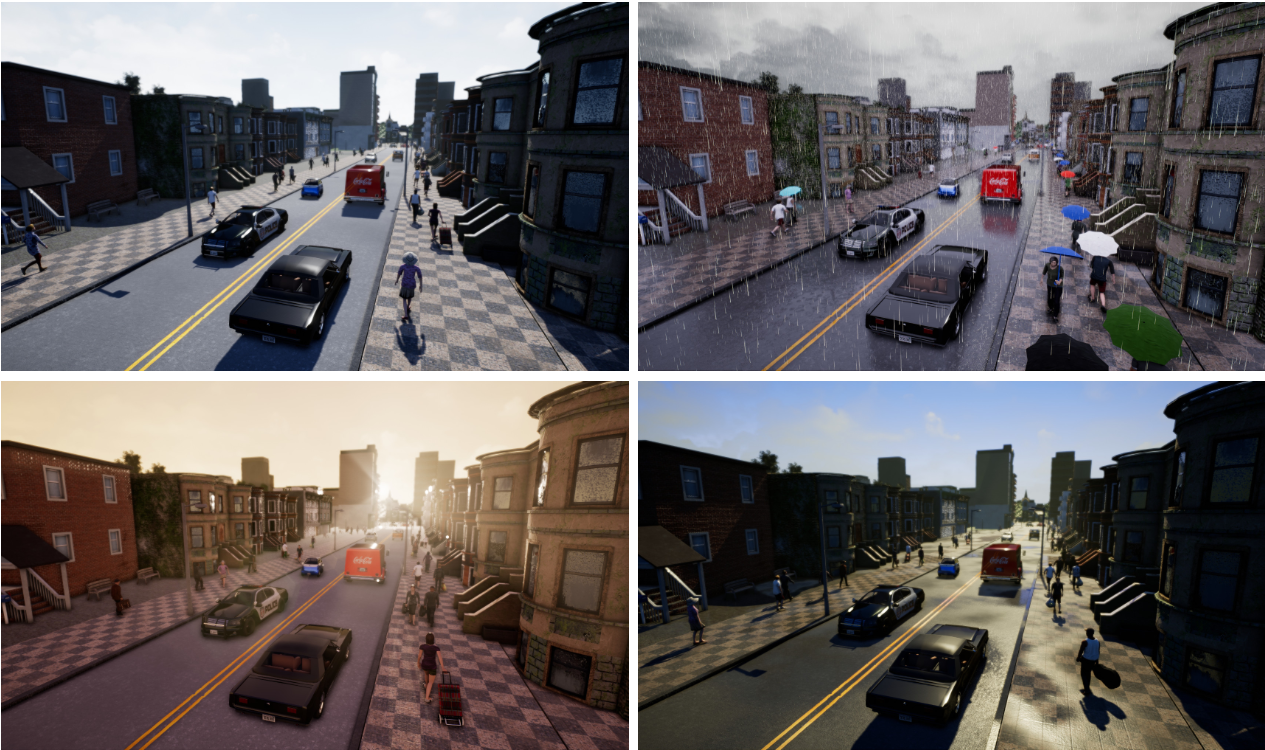
\includegraphics[width=0.8\textwidth]{img/carla_clima_example}
	\caption{Ejemplos de condiciones ambientales configurables en el simulador CARLA.}
	\label{fig:carla-simulator-teo}
\end{figure}

\subsubsection{OpenCV}
\noindent
OpenCV proporciona el conjunto de operaciones y estructuras necesarias para el preprocesado de imágenes y la extracción de primitivas geométricas, incluyendo umbralización, Canny y la transformada de Hough, que se emplean en la detección de la retícula de estacionamiento.

\subsubsection{scikit-learn: \texttt{AgglomerativeClustering}}\label{sec:sklearn-agglomerative}
\noindent
Para la agrupación de intersecciones utilizamos el algoritmo de \emph{clustering} jerárquico aglomerativo provisto por \texttt{scikit-learn}.
Este enfoque construye una jerarquía de fusiones de abajo hacia arriba, uniendo en cada paso los grupos más próximos según
una métrica de distancia y un criterio de enlace (\texttt{linkage} en \{\texttt{ward}, \texttt{complete}, \texttt{average}, \texttt{single}\}).
El parámetro \texttt{distance\_threshold} permite dejar que el propio algoritmo determine el número de clusters deteniendo
las fusiones cuando la distancia supera un umbral, lo cual resulta práctico en escenas con variabilidad de densidad.
Esta técnica es apropiada para consolidar intersecciones cercanas al horizonte en cúmulos cuya localización (centroide)
sirve de estimación inicial de puntos de fuga \cite{tan2005introduction}.

\subsubsection{Herramienta de experimentación y ajuste de parámetros}\label{sec:experimentation-tool}
\noindent
Para determinar la configuración óptima de parámetros de la solución propuesta, se desarrolló una aplicación en Python
que carga una secuencia de imágenes de la trayectoria del vehículo en el estacionamiento y, para cada cuadro,
calcula la retícula aplicando los pasos descritos en este trabajo. La herramienta permite visualizar el resultado de cada
etapa y ajustar dinámicamente los parámetros para analizar su impacto en tiempo real.

\noindent
Parámetros ajustables considerados:
\begin{itemize}
	\item \texttt{threshold\_image}: Umbral de binarización de la imagen.
	\item \texttt{canny\_threshold\_1}: Umbral inferior para Canny.
	\item \texttt{canny\_threshold\_2}: Umbral superior para Canny.
	\item \texttt{hough\_rho}: Resolución de distancia (píxeles) en Hough.
	\item \texttt{hough\_theta}: Resolución angular (radianes) en Hough.
	\item \texttt{hough\_threshold}: Umbral de votos en Hough.
	\item \texttt{hough\_min\_line\_length}: Longitud mínima de segmento.
	\item \texttt{hough\_max\_line\_gap}: Máxima separación para unir segmentos.
	\item \texttt{relevant\_intersections\_horizon\_threshold}: Umbral de cercanía al horizonte.
	\item \texttt{agglomerative\_distance\_threshold}: Distancia máxima para pertenecer al mismo cúmulo.
\end{itemize}

\noindent
A modo ilustrativo, a continuación  en la figura \ref{fig:experimentationBinary-teo} 
se muestra la herramienta donde se visualizan contornos, líneas detectadas,
intersecciones, intersecciones relevantes, cúmulos y puntos de fuga.

\begin{figure}[!ht]
	% \begin{subfigure}{0.5\textwidth}
	% 	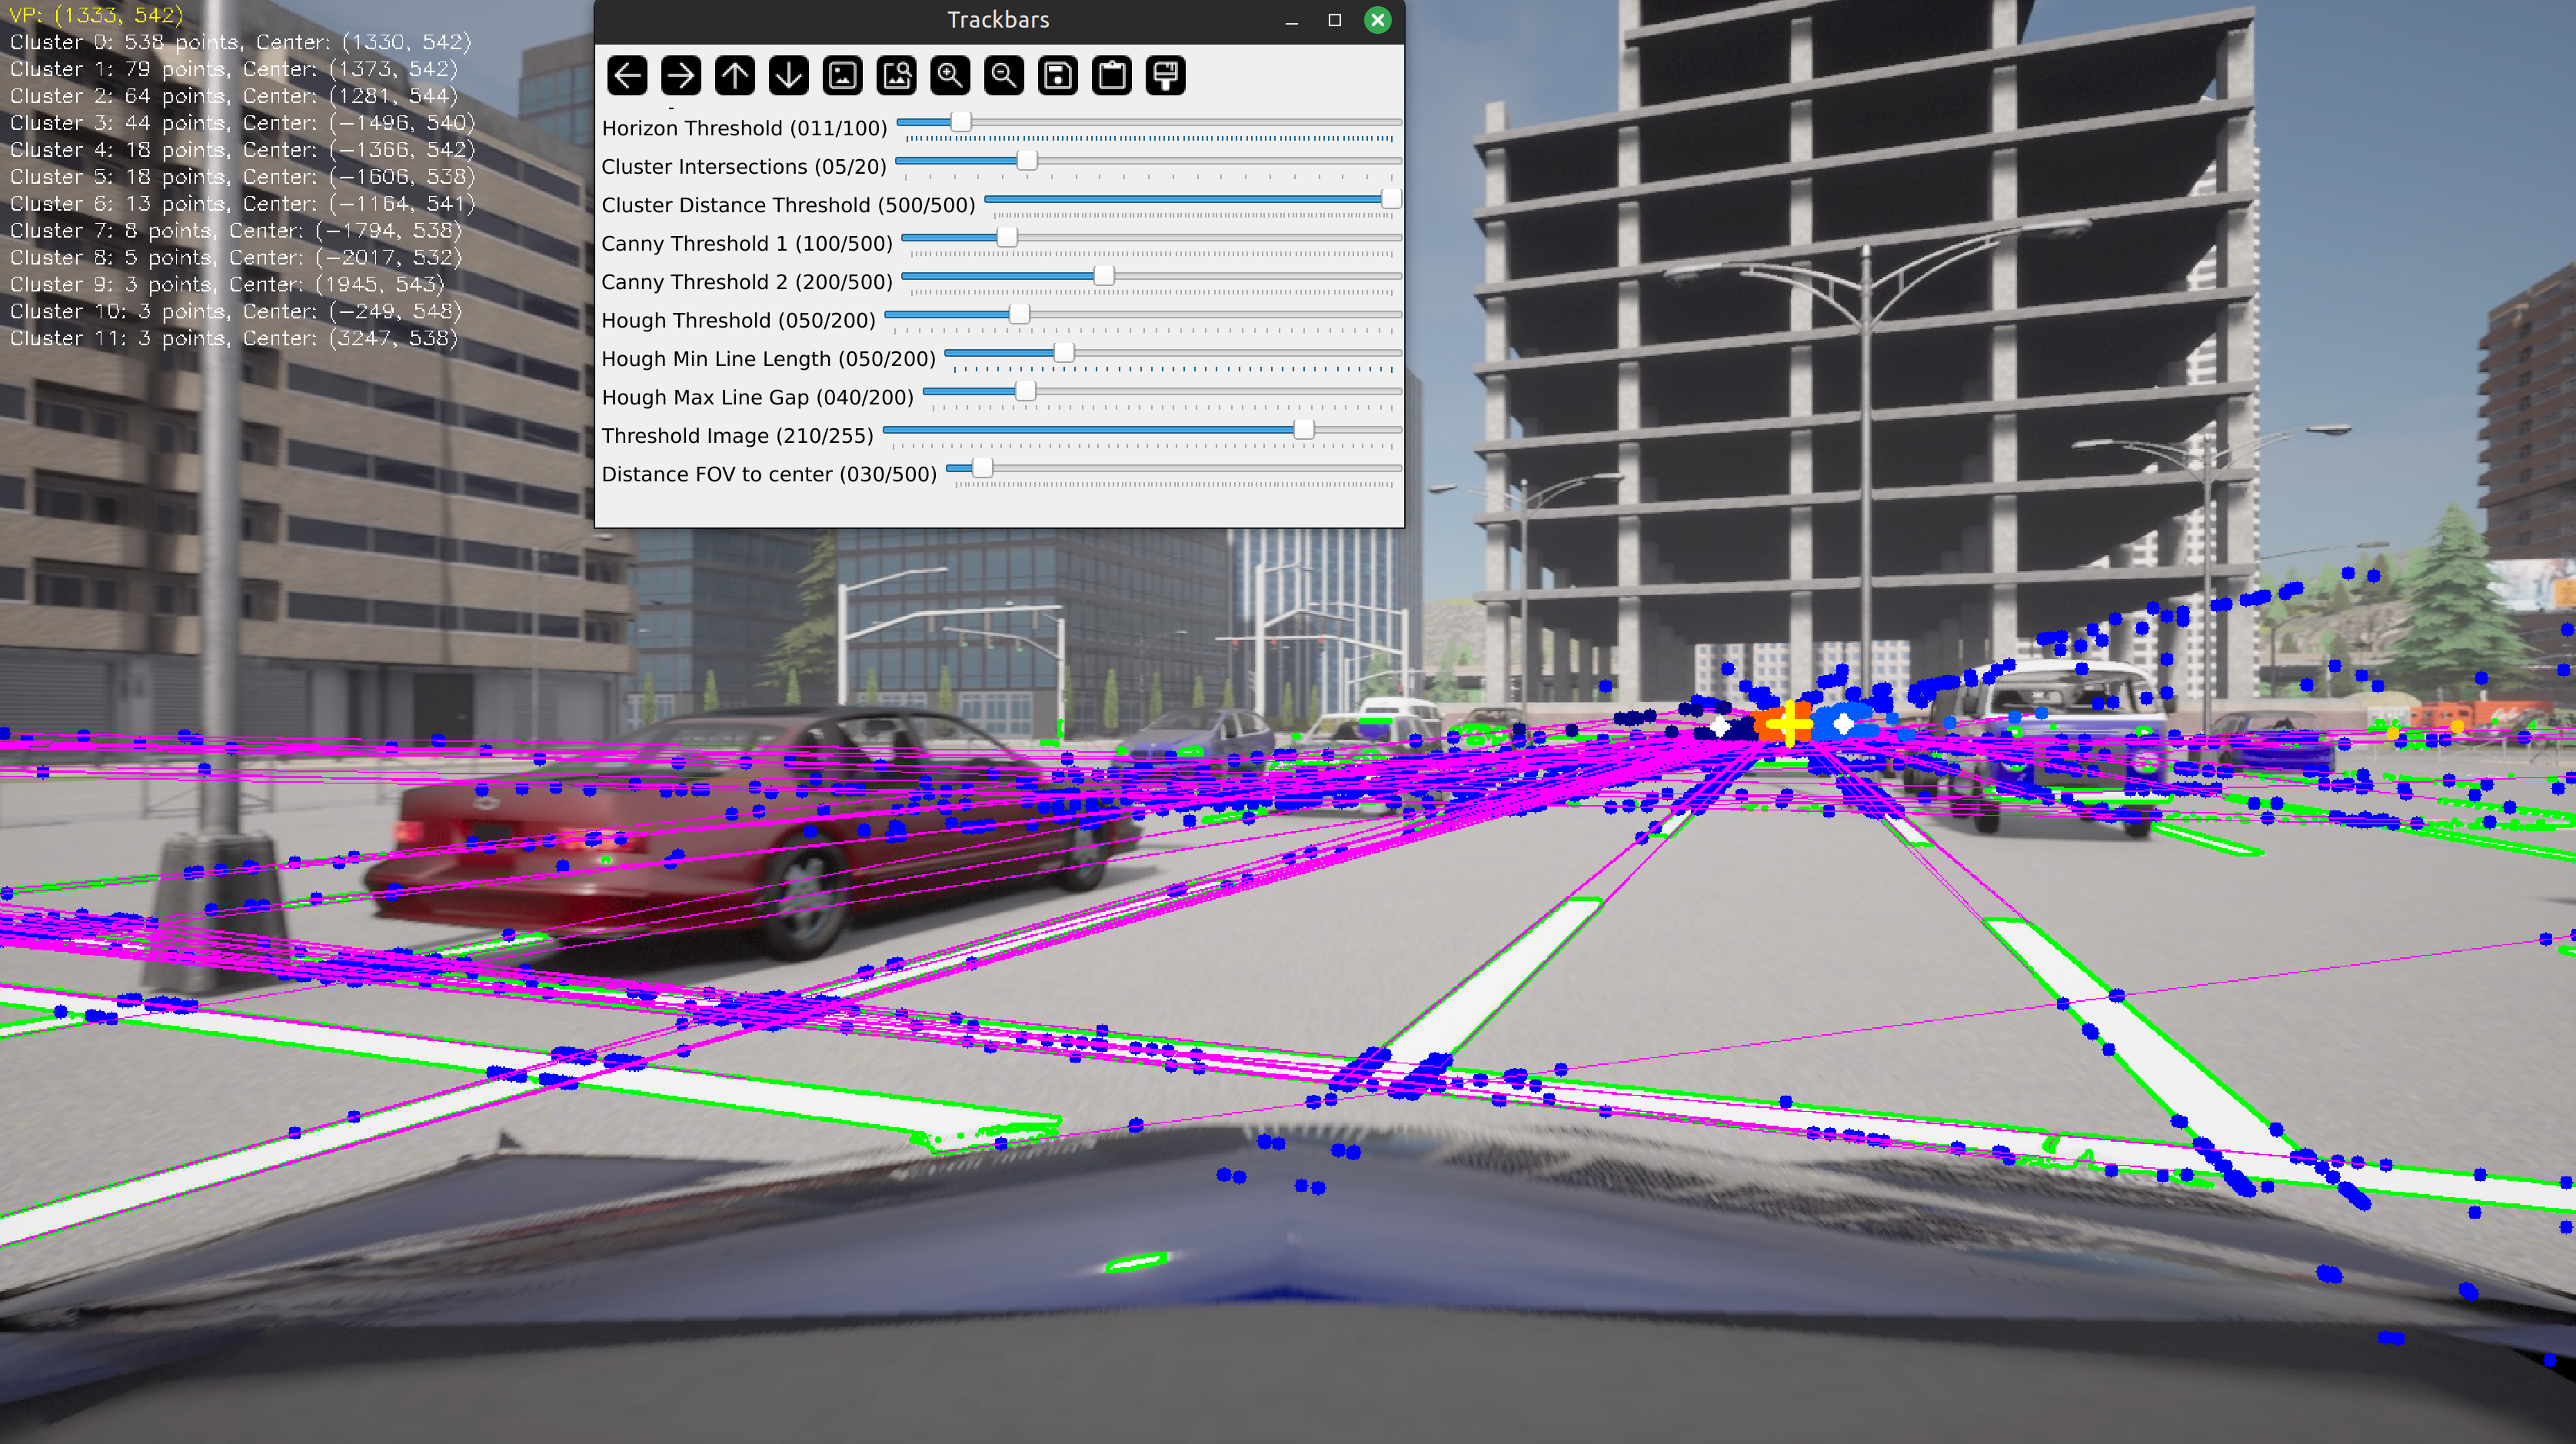
\includegraphics[width=\textwidth]{img/reticule/experimentationRgb}
	% 	\caption{Ejemplo de experimentación (RGB)}
	% 	\label{fig:experimentationRgb-teo}
	% \end{subfigure}
	
		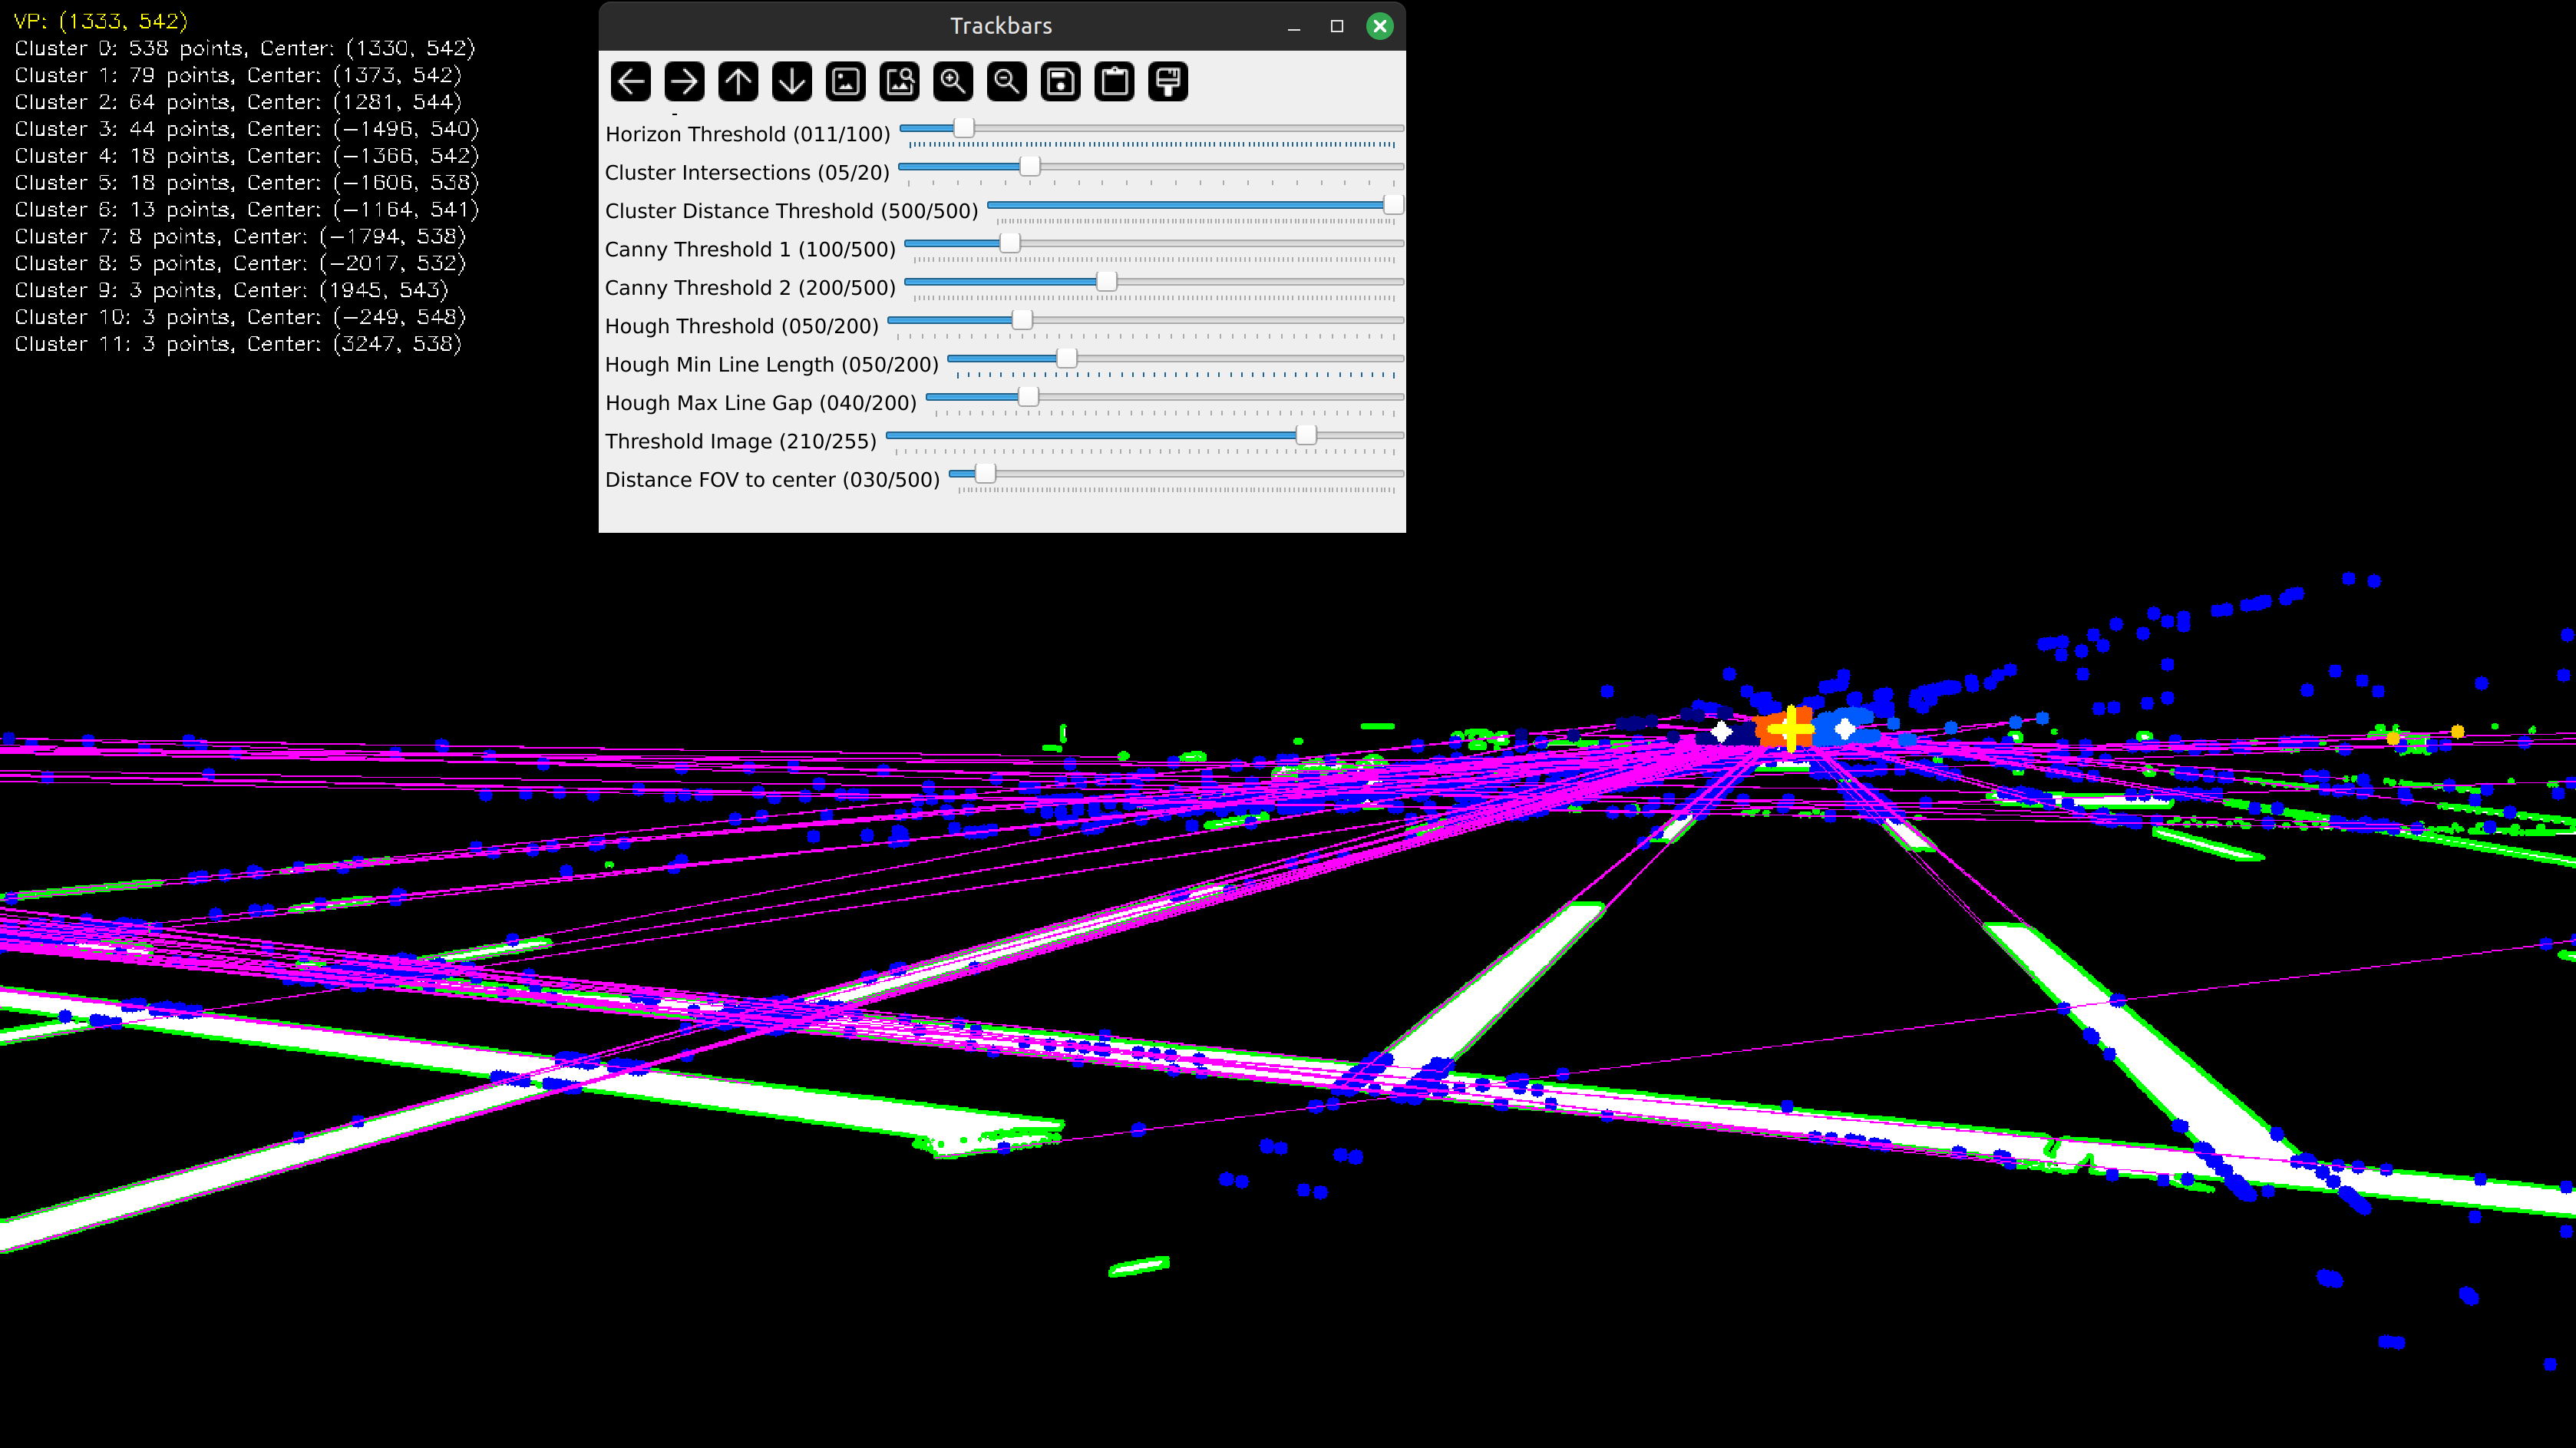
\includegraphics[width=0.8\textwidth]{img/reticule/experimentationBinary}
		\caption{Ejemplo de experimentación (Binaria)}
		\label{fig:experimentationBinary-teo}
	
\end{figure}

\noindent
La interfaz incorpora una "Trackbar" para modificar parámetros en tiempo real y observar su efecto inmediato,
facilitando la búsqueda de configuraciones estables y robustas para distintas condiciones de escena.
